\documentclass[11pt,letterpaper]{article}

\usepackage[margin=1.1in]{geometry}
\usepackage{amsmath,amssymb}
\usepackage{graphicx}
\usepackage{booktabs}
\usepackage{hyperref}
\usepackage{caption}
\usepackage{enumitem}
\usepackage{float}

\hypersetup{colorlinks=true,linkcolor=black,citecolor=black,urlcolor=blue,
  pdftitle={IRIS-Harness: Harness-level Recursive Self-Improvement for Image Restoration},
  pdfauthor={zram}}

\title{\bfseries IRIS-Harness: Harness-level Recursive Self-Improvement\\
for Image Restoration with Self-Improvement Memory}
\author{zram}
\date{2026}

\begin{document}
\maketitle

\begin{abstract}
Most image restoration pipelines are tuned by repeatedly retraining or redesigning the
backbone, yet performance often depends as much on the surrounding inference harness---
pre-processing, backend selection, post-processing, test-time augmentation, and evaluation
protocol---as on the model weights. We present \textbf{IRIS-Harness}, a harness-level
recursive self-improvement framework for low-level vision restoration. The restoration
backbone is kept frozen; the framework instead evolves a configurable outer harness through
a closed Proposer--Selector--Evaluator loop. A structured \textbf{Self-Improvement Memory
(SIM)} records, per degradation root cause, each harness edit together with its rationale,
predicted outcome, observed outcome, verdict, and provenance; both successful and failed
edits are retained so that later rounds prune known regressions and reuse known improvements
across backends. On four real paired benchmarks covering low-light enhancement, dehazing,
underwater enhancement, and denoising, the evolved harness improves low-light PSNR by
\textbf{+3.73\,dB} and SSIM by \textbf{+0.049}, improves dehazing SSIM by \textbf{+0.011}
while reducing color shift and output variance, and improves underwater PSNR by
\textbf{+0.77\,dB} and SSIM by \textbf{+0.051}; on denoising the protocol honestly retains
the baseline when no peripheral edit helps.
\end{abstract}

\section{Introduction}
\label{sec:intro}

Image restoration and enhancement---dehazing, low-light enhancement, underwater color
correction, and denoising---remain core low-level vision tasks. A large body of work designs
ever stronger backbone networks, and recent self-improvement studies in vision concentrate
on weight tuning, architecture search, or loss redesign. In practice, however, a deployed
restoration system is wrapped by an outer harness: white-balance and gamma pre-processing,
the choice of enhancement backend, gain/color-curve/sharpening post-processing, test-time
augmentation, and the evaluation protocol that decides whether a change is an improvement.
When the degradation type, the backbone, or the evaluation set changes, this harness often
has to be re-tuned by hand, and previously discovered fixes are rarely transferred
systematically.

Our starting observation is that the harness is itself a searchable object, and that its
edits are cheaper to evaluate than backbone retraining. Borrowing the Continual Recursive
Self-Improvement (CRSI) idea from the agent-harness setting, we treat the frozen restoration
model as an inner policy and optimize the outer harness recursively. Two ingredients are
specific to the image restoration domain:

\begin{itemize}[leftmargin=*]
  \item A \textbf{root-cause-driven candidate space}: harness edits are organized around
        observable failure causes (dark, bright, low contrast, color cast, haze residual),
        so that a proposed change is attributable to a specific peripheral component.
  \item A \textbf{structured Self-Improvement Memory (SIM)}: every edit stores its predicted
        and measured effect on PSNR, SSIM, and color shift, together with a verdict. Failed
        edits are kept, not discarded, and are used to prune candidates in later rounds.
\end{itemize}

Our contributions are: (i) a harness-level recursive self-improvement framework dedicated to
image restoration, with frozen backends and a configurable pre/backend/post pipeline;
(ii) a SIM design that transfers successful and failed peripheral edits across degradation
types and backends; and (iii) validation on four real paired benchmarks, with an honest
account of tasks where the harness cannot improve over the baseline.

\section{Related Work}
\label{sec:related}

\textbf{Lightweight restoration backends.} Zero-DCE~\cite{guo2021zerodce} estimates pixel-wise
tone curves with a small seven-layer CNN for low-light enhancement. FUnIE-GAN~\cite{islam2020funie}
uses a five-layer UNet conditional GAN generator for real-time underwater enhancement.
AOD-Net~\cite{li2017aodnet} formulates dehazing as a lightweight transmission estimation
network. Classical operators---gray-world white balance, CLAHE, multi-scale Retinex, bilateral
filtering, and non-local means~\cite{buades2005nlm}---provide parameterized no-weight baselines.
We wrap these models behind one unified frozen-backend interface rather than training any of
them.

\textbf{Harness and recursive self-improvement.} Recent agent studies show that, with a fixed
policy model, the harness (prompt, tools, execution flow, evaluation) can be improved
recursively, and that a self-improvement memory accumulates reusable edits across tasks and
models~\cite{crsi2026sim}. We adapt this paradigm to computer vision: the ``policy model'' is
the frozen restoration backbone, and the harness is the image pipeline and its evaluation
protocol.

\textbf{Automated pipeline search.} Neural architecture search and AutoISP methods search
network structure or ISP parameters end-to-end. In contrast, IRIS-Harness leaves weights
untouched and searches only the peripheral harness, which is cheaper, more interpretable, and
directly compatible with deployable frozen checkpoints.

\section{Method}
\label{sec:method}

\subsection{Problem Formulation}
Let $f_\theta$ denote a frozen restoration backbone with fixed weights $\theta$. A harness
$h = (p, b, q)$ composes a pre-processor $p$, a selected backend $b$, and a post-processor
$q$. For a degraded image $x$ with reference $y$, the harness produces
$\hat{y} = q\big(b\,(p(x))\big)$. Given an evaluation metric $M$, the harness-level objective
is
\begin{equation}
  h^* = \arg\max_{h \in \mathcal{H}} \; M\big(E(h(x)), y\big),
\end{equation}
where $\mathcal{H}$ is the discrete candidate space of peripheral edits and $E$ is the
evaluation protocol. The backbone $\theta$ is never updated.

\subsection{Tunable Harness Components}
The candidate space covers peripheral components only:
\begin{itemize}[leftmargin=*]
  \item \textbf{Pre-processing}: gray-world white balance, gamma correction, percentile
        contrast stretch.
  \item \textbf{Backend selection}: switching among the registered frozen backends for a task.
  \item \textbf{Post-processing}: linear gain, gamma curve, per-channel gain (color cast
        correction), unsharp masking, and horizontal-flip TTA averaging.
  \item \textbf{Backend parameters}: denoising filter strength where applicable.
\end{itemize}
Edits are emitted as single-factor changes (with a small number of two-factor combinations)
so that any observed metric change can be attributed to one harness component.

\subsection{Self-Improvement Memory (SIM)}
Each memory entry records: the degradation type and backbone, the root cause, the harness edit
(stage, key, old value, new value), the rationale, the predicted outcome, the observed
aggregate metrics, a verdict, and provenance (round, subset, sample count, baseline metrics).
Entries are persisted to JSON and resumable. Two retrieval modes are used:
\begin{itemize}[leftmargin=*]
  \item \textbf{Regression pruning}: previously \texttt{regressed} $(key, value)$ pairs for
        the same degradation are removed from later candidate sets.
  \item \textbf{Improvement reuse}: previously \texttt{improved} pairs are ranked first.
\end{itemize}
Retrieval does not filter by backbone, so peripheral experience transfers across
backends.

\subsection{Closed Loop}
The runner alternates three roles per task:
\begin{description}[leftmargin=*]
  \item[Proposer.] Analyzes failure statistics (mean brightness, contrast, color ratio) to
        attach root causes, then proposes single-factor edits from the task candidate space.
  \item[Selector.] Queries SIM to prune known regressions and prioritize known improvements.
  \item[Evaluator.] Scores retained candidates on the hard subset (worst 50\% by PSNR) using a
        composite score and hard-regression guards, then re-evaluates the winning harness on
        the full set.
\end{description}
The composite score is
\begin{equation}
  s = 0.5\,\frac{\Delta\mathrm{PSNR}}{10}
    + 0.3\,\frac{\Delta\mathrm{SSIM}}{0.2}
    - 0.2\,\frac{\Delta\mathrm{Shift}}{20}.
\end{equation}
A candidate is marked \texttt{regressed} directly when PSNR drops by more than $0.3$\,dB, or
SSIM by more than $0.01$, or color shift rises by more than $3.0$. A \textbf{full-set rollback
guard} rejects a hard-subset improvement that regresses significantly on the full set, and
writes the failure back to SIM.

\subsection{Frozen Backends}
\begin{table}[H]
\centering
\caption{Frozen backends wrapped by IRIS-Harness.}
\label{tab:backends}
\begin{tabular}{lcll}
\toprule
Backend & Task & Params & Type \\
\midrule
Zero-DCE & Low-light & 79.4k & Deep CNN \\
FUnIE-GAN & Underwater & 7.02M & UNet GAN \\
AOD-Net & Dehazing & 1.8k & Deep CNN \\
GrayWorld / CLAHE / MSR / Bilateral / NLM & WB / Contrast / Denoise & 0 & Classical \\
\bottomrule
\end{tabular}
\end{table}

\section{Experiments}
\label{sec:exp}

\subsection{Datasets}
\begin{table}[H]
\centering
\caption{Real paired benchmarks used for evaluation.}
\label{tab:datasets}
\begin{tabular}{llcl}
\toprule
Task & Dataset & Pairs & Protocol \\
\midrule
Low-light & LOL test (paired) & 15 & Real low-light / normal exposure pairs \\
Dehazing & RESIDE-style paired set & 100 & Clear image + atmospheric haze \\
Underwater & EUVP paired, 256$\times$256 & 40 & Real underwater / normal pairs \\
Denoising & Kodak24 + Gaussian noise $\sigma{=}25$ & 24 & Clean image, noise added on the fly \\
\bottomrule
\end{tabular}
\end{table}

\subsection{Metrics and Protocol}
We report paired PSNR (dB), SSIM, and mean per-channel color shift (lower is better), with
mean$\pm$std over each full test set. The closed loop runs for two rounds; candidates are
first judged on the hard subset and the winner is re-evaluated on the full set.

\subsection{Main Results}
\begin{table}[H]
\centering
\caption{Baseline harness vs.\ evolved harness on the full real test sets (mean$\pm$std).
``Shift'' is mean per-channel color shift.}
\label{tab:results}
\begin{tabular}{llcccccc}
\toprule
Task & Backend & PSNR B & PSNR E & SSIM B & SSIM E & Shift B & Shift E \\
\midrule
Low-light & zero\_dce & 14.94$\pm$4.29 & \textbf{18.67$\pm$4.30} & 0.653 & \textbf{0.702} & 45.64 & \textbf{25.84} \\
Dehazing & aodnet & 21.08$\pm$3.40 & 21.07$\pm$2.04 & 0.897 & \textbf{0.909} & 12.87 & \textbf{10.68} \\
Underwater & funie\_gan & 19.45$\pm$3.28 & \textbf{20.21$\pm$3.46} & 0.752 & \textbf{0.803} & 13.16 & 13.23 \\
Denoising & nlm & 24.80$\pm$1.71 & 24.80$\pm$1.71 & 0.647 & 0.647 & 1.38 & 1.38 \\
\bottomrule
\end{tabular}
\end{table}

The evolved low-light harness combines post gain $1.35$ with gamma $0.7$, raising PSNR by
\textbf{+3.73\,dB}, SSIM by \textbf{+0.049}, and cutting color shift by $19.80$. The evolved
dehazing harness applies gamma $1.15$ with an R-channel gain of $0.92$; mean PSNR is essentially
unchanged ($-0.01$), but SSIM rises by $0.011$, color shift drops by $2.20$, and the PSNR
standard deviation shrinks from $3.40$ to $2.04$, i.e.\ the worst cases are pulled back toward
the reference. The evolved underwater harness uses horizontal-flip TTA averaging, improving
PSNR by \textbf{+0.77\,dB} and SSIM by \textbf{+0.051}. On denoising, all alternative backends,
filter strengths, and sharpening edits regressed or were neutral; the baseline NLM output
already has near-zero channel bias ($\approx[-2.2,-1.5,0]$), so the protocol honestly retains
the baseline.

\subsection{Memory and Loop Analysis}
Across two rounds, SIM accumulates \textbf{45} entries: \textbf{7} improved, \textbf{22}
regressed, and \textbf{16} neutral. In the second round the Selector prunes \textbf{15}
previously regressed $(key, value)$ candidates, avoiding repeated trials. A residual analysis
of the dehazing baseline revealed a systematic over-bright, red-shifted output
($+14.6/+8.5/+6.2$ channel bias); the original candidate space only contained brightening
gains, so adding a darkening gamma axis and an R-channel suppression axis was required before
the loop could find the improving direction. This case illustrates how root-cause diagnosis
extends the candidate space itself.

\begin{figure}[H]
\centering
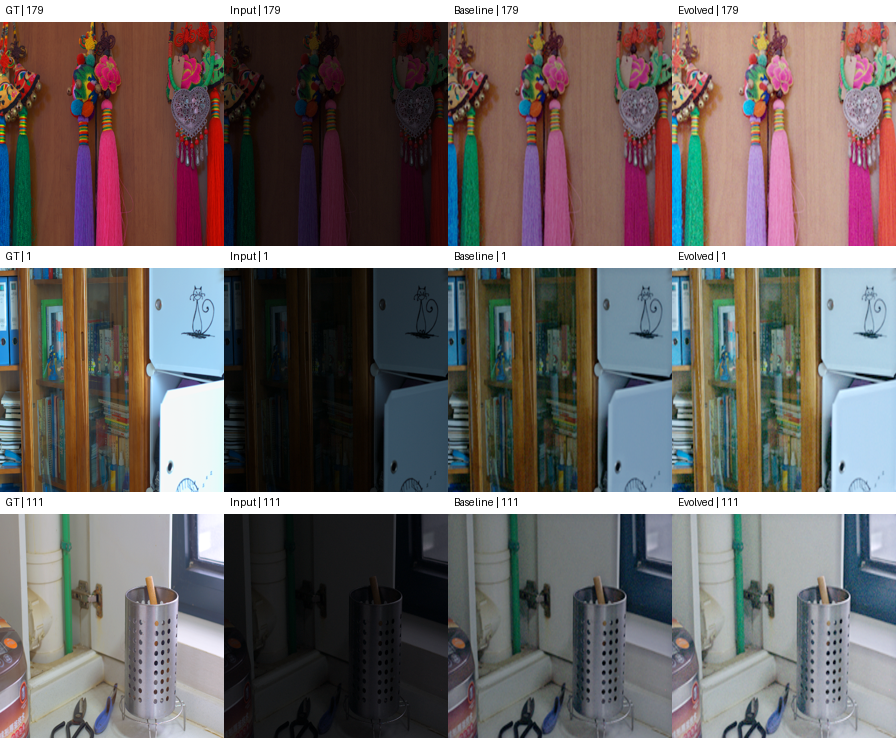
\includegraphics[width=0.92\columnwidth]{fig/fig_lowlight.png}
\caption{Low-light comparison (GT / Input / Baseline / Evolved). The evolved gain+gamma
harness recovers detail and color closer to the reference.}
\label{fig:lowlight}
\end{figure}

\begin{figure}[H]
\centering
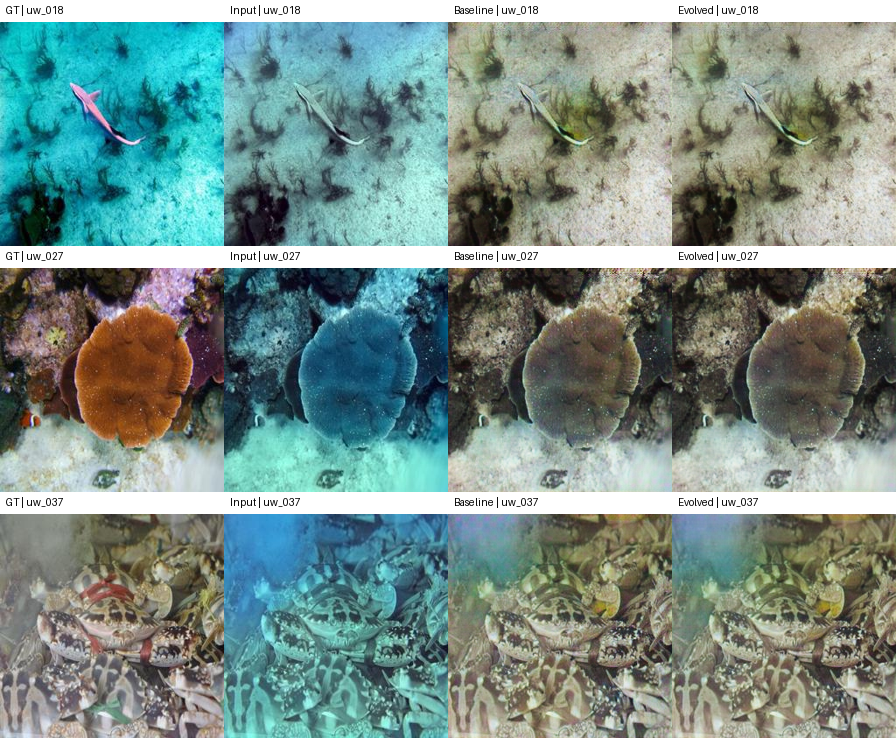
\includegraphics[width=0.92\columnwidth]{fig/fig_underwater.png}
\caption{Underwater comparison (GT / Input / Baseline / Evolved). Flip-TTA averaging yields
a stabler structure and closer SSIM to the reference; residual warm cast is set by the frozen
backbone.}
\label{fig:underwater}
\end{figure}

\section{Limitations}
\label{sec:lim}

The deep backends are lightweight legacy models, and the ceiling of some tasks is set by the
frozen backbone rather than the harness. Classical denoising/dehazing alternatives are weak;
stronger frozen backends such as RIDNet or lightweight Transformers can be plugged in for
comparison. Metrics do not yet include LPIPS, CLIP-IQA, or subjective scoring, and the
candidate space remains single-factor plus a few two-factor combinations. The underwater set
is a 40-pair sample; full EUVP and additional benchmarks (UIEB, SID, SOTS) are future work.

\section{Conclusion}
\label{sec:conclusion}

We presented IRIS-Harness, a harness-level recursive self-improvement framework for image
restoration. Keeping the backbone frozen, the loop evolves pre/post-processing, backend
selection, and TTA around a structured SIM that transfers both successful and failed peripheral
edits across rounds and backends. On four real paired benchmarks the evolved harness improves
low-light, dehazing, and underwater restoration, while the protocol retains the baseline where
no peripheral edit helps. The framework is backend-agnostic and intended as a testbed for
harness-level optimization and ablation automation in low-level vision.

\begin{thebibliography}{9}
\bibitem{guo2021zerodce}
Guo, C., Li, C., Guo, J., et al. \emph{Zero-Reference Deep Curve Estimation for Low-Light
Image Enhancement}. CVPR, 2021.

\bibitem{islam2020funie}
Islam, M. J., Xia, Y., Sattar, J. \emph{Fast Underwater Image Enhancement for Improved Visual
Perception}. IEEE Robotics and Automation Letters (RA-L), 2020.

\bibitem{li2017aodnet}
Li, B., Peng, X., Wang, Z., Xu, J., Feng, D. \emph{AOD-Net: All-in-One Dehazing Network}.
ICCV, 2017.

\bibitem{buades2005nlm}
Buades, A., Coll, B., Morel, J.-M. \emph{A Non-Local Algorithm for Image Denoising}. CVPR, 2005.

\bibitem{crsi2026sim}
Yu, X., Xia, F., Tang, J., et al. \emph{Self-Improvement Memory Enables Continual Recursive
Self-Improvement}. arXiv:2611.18856, 2026.

\bibitem{lore2017lol}
Lore, K. G., Akintayo, A., Sarkar, S. \emph{LLENet: A Deep Autoencoder Approach to Low-Light
Image Enhancement}. Pattern Recognition Letters, 2017.
\end{thebibliography}

\end{document}
